\chapter{深度伪造与检测的背景}
\label{chap:1}
近年来人工智能与深度学习等计算机学科的蓬勃发展,连带也造成的不同研究领域与多样的议题需要进行研讨,比如讨论在以人工智慧应有的社会治理架构下,讨论其机器学习领域等演算法等对于法学所造成的挑战\cite{law01},同时另一篇研究也讨论其人工智能与演算法在法律上应用的可能 \cite{law03}。而在机器学习领域下的深度伪造技术则发展有越来越广泛的趋势,而其深度伪造属于机器学习下的深度学习的一部分,而深度学习已经广泛应用于各个领域,其领域包含了计算机视觉与自然语言处理,而本作业则关注当中快速兴起的则是深度伪造的领域,其深度伪造技术\cite{list1101}虽造成了风险,但同时在这些年也有需多研究去分析深度伪造的工作原理,并且引入了许多基于深度学习的方法来检测深度伪造的影像或图像。

综上所述这些技术好的部分则是应用于将古老的照片变成动态的影像,或者是用于一些艺术与网路次文化的创作,又或者是 Reface APP\cite{list1102} 等服务带给大众娱乐,但同时负面的因素也有造成社会动荡的可能,包含知名人士被伪造影像、近而被广泛散布不实资讯与谣言的危险,造成当事人的声誉、社会地位与事业严重打击,还有近期大量知名女姓人士被用于成人色情网站,而受害当事人却因执法基层人员不理解相对应技术亦或是没有完善的检测工具,因而在此方面无法给予有效的协助,而受害人在描述其受害过程时受到再次的心理创伤,同时其深度伪造的假影片在网路散布时,对当事人的伤害就已经造成。再者此技术近期被应用在战争宣传战,将敌对方的政治人物伪造出用于其不正确的政治发言影片,进而造成某方的士气遭到打击。

\begin{figure}[htb]
\centering 
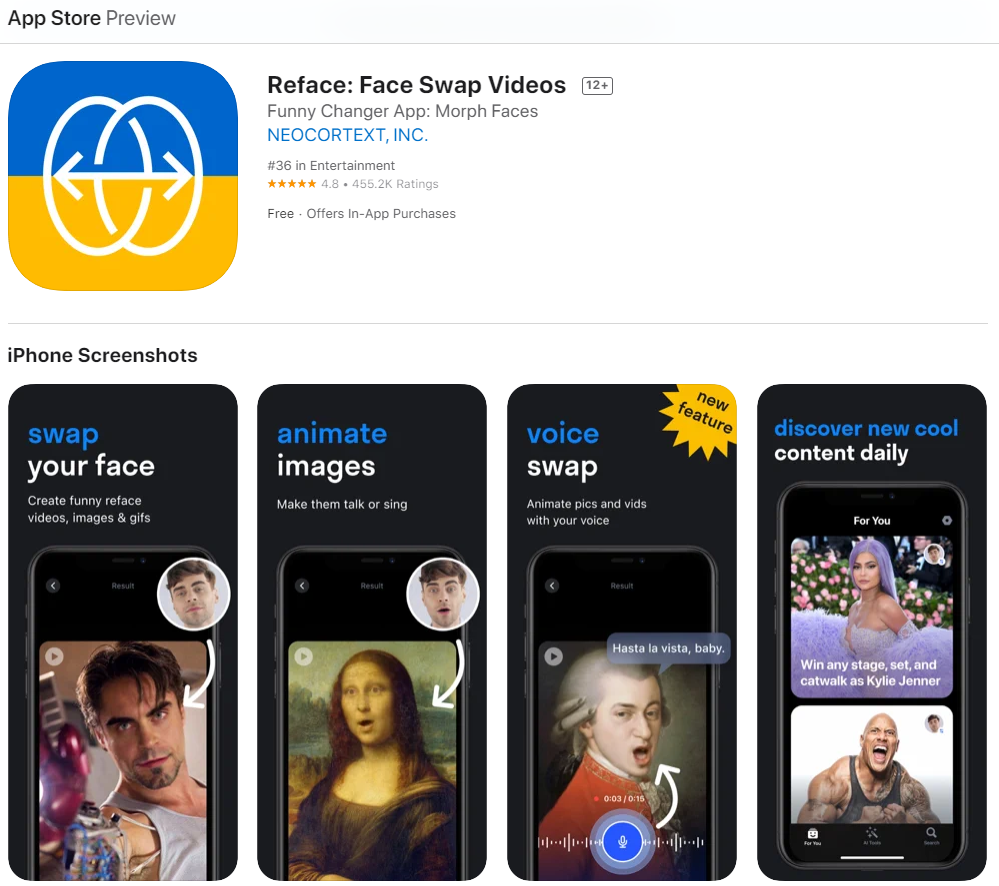
\includegraphics[width=0.40\textwidth]{img/ch1m1.png} 
\caption{Reface APP 苹果商店页面}
\label{Test}
\end{figure}

另外需要注意的在于这些工具非常容易取得,与之相应的是一些相继机构发现这些问题后,进而举办相应的竞赛\cite{list1103},来推广该技术在此领域的热度。所以本作业即目标即探讨在人工智能下的深度学习领域中深度伪造与其检测的研究整理,同时调研过去Girish N 等人所汇整的早期图像篡改工作 \cite{girish2019review}与 Nguyen TT 等人 对该领域工作地早期总结 \cite{nguyen2019deep}与 Li XR 等人近期来的汇整工作\cite{2021496} 与研读,同时对使用深度学习方法下深度伪造与相对应的前沿检测技术进行调查,并对目前最新的研究进行补充。

\section{深度伪造技术}

目前对深度伪造技术在视觉上所修改后的影像与图片,其大多是针对人类脸部的替换。而在此大致分为两大部分,其一为对人类的人脸表情进行伪造,让指定窜改者所改造的对象做到窜改者想要的脸部表情与动作,但不对该人脸进行目标人脸的替换,另一类则是根据两个不同影像与影片的人脸进行替换,经过将另一个完全不同身份的人脸替换过去,从而达到该内容目标人物是窜改者所要之人。该技术从过往运用的三维重建技术等方法来修改之外,一路发展到运用深度学习的方法至今则用生成对抗网路为基础进行仿造,比如 Almars, A. M 等人在该领域工作汇整之一的 CycleGAN,此方法为无监督方法,它提取一张图像的特征,并通过 GAN 架构生成另一张具有相同特征的图像。该方法应用循环损失函数,使他们能够学习潜在特征,且该方法应用循环损失函数,使他们能够学习潜在特征,可以在不使用配对示例的情况下执行图像到图像的转换。换句话说,该模型从源和目标中学习不需要相互关联的图像集合的特征。而更重要的是目前的仿造技术还运用人类语音的修改,从而导致伪造出来的影像结果会更逼真。

\begin{figure}[htb]
\centering 
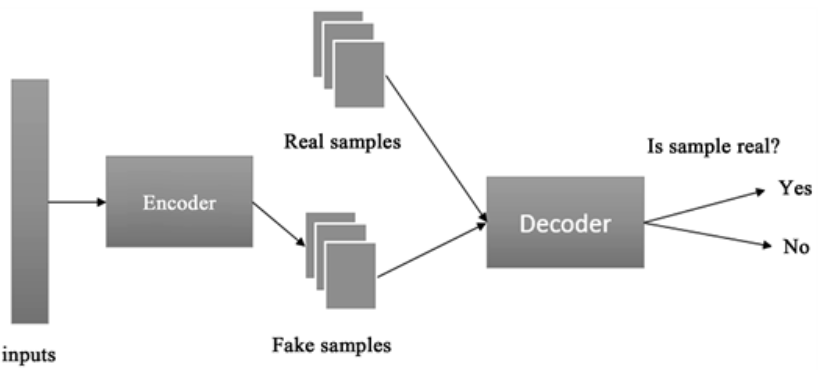
\includegraphics[width=0.70\textwidth]{img/ch1m2.png} 
\caption{Almars, A. M 等人整理的 GAN 深度伪造示意}
\label{Test}
\end{figure}

\subsection{针对人类脸部的伪造技术}

\subsubsection{过往根据图形学所进行的脸部伪造技术}

在过往几年来使用图形学来对人类的脸部进行替换和仿造的技术,一直被很多研究者持续的关注,而在 Zollhöfer M 等人对其领域进行调研总结的工作则说明地当下几个主要根据三维模型重建与追踪再该领域技术上的应用。该研究将讨论重点放在中心任务是使用基于优化的重建算法来恢复和跟踪人脸的三维模型的方法上,同时对现实世界图像形成的基本概念进行了深入的概述,并讨论了使这些算法实用的常见假设和简化。此外,该研究广泛涵盖了用于更好地约束欠约束单目重建问题的先验,并讨论了用于从单目 2D 数据中恢复密集的照片几何 3D 人脸模型的优化技术。最后,在动作捕捉、面部动画以及图像和视频编辑的背景下讨论了所审查算法的各种用例。

而 FaceSwap \cite{list1107} 是一个根据图形学的人脸替换方法,该应用是 Marek Kowalski 于华沙理工大学就读多媒体数学时,所做的练习成果,其应用程序是用 Python 编写的,并使用人脸对齐、高斯牛顿优化和图像混合来将相机看到的人脸与提供的图像中的人脸交换。同时该应用的新版本则基于深度对齐网络方法,如果在 GPU 上运行,它比当前使用的方法更快,并且提供更稳定和更精确的面部标志。另外 Dale K 等人\cite{dale2011video}提出了一种替换视频中人类脸部的方法,该研究的方法考虑了源视频和目标视频之间在身份、视觉外观、语音和时间方面的差异。该研究与以前的工作不同,它不需要大量的手动操作或复杂的采集硬件,只需要单机视频,研究者使用 3D 多线性模型来跟踪两个视频中的面部表现,使用相应的 3D 几何,最后将源扭曲到目标面并重新定时源以匹配目标性能。然后,研究者通过视频体积计算最佳接缝,以保持最终合成中的时间一致性。

\begin{figure}[htb]
\centering 
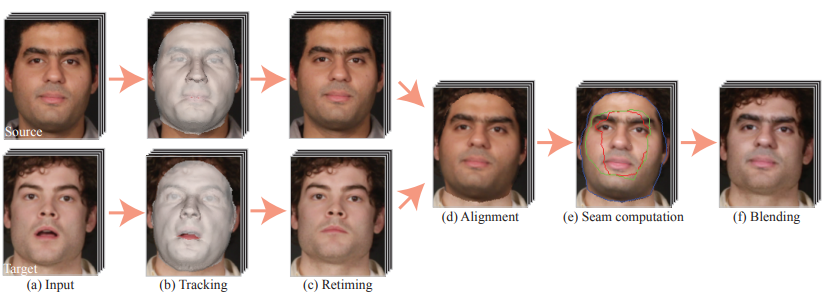
\includegraphics[width=0.70\textwidth]{img/ch1m3.png} 
\caption{Dale K 等人一种基于图像的面部重建系统}
\label{Test}
\end{figure}

Garrido P \cite{garrido2014automatic} 等人则研究提出了一种基于图像的面部重建系统,该系统将现有目标视频中的演员面部替换为源视频中用户的面部,同时保留原始目标表现,其系统是全自动的,不需要源表达式数据库。相反,它能够从使用现成相机(例如网络摄像头)捕获的短源视频中产生令人信服的重演结果,用户在其中执行任意的面部表情,研究者的重演流程被设想为部分图像检索和部分面部转移:图像检索基于目标帧的时间聚类和一种新颖的图像匹配度量,该度量结合了外观和运动以从源视频中选择候选帧,而面部转移使用保留用户身份的 2D 变形策略。其系统在简单性方面表现出色,因为它不依赖于 3D 人脸模型,它在头部运动下很稳健,并且不需要源和目标性能相似。

\begin{figure}[htb]
\centering 
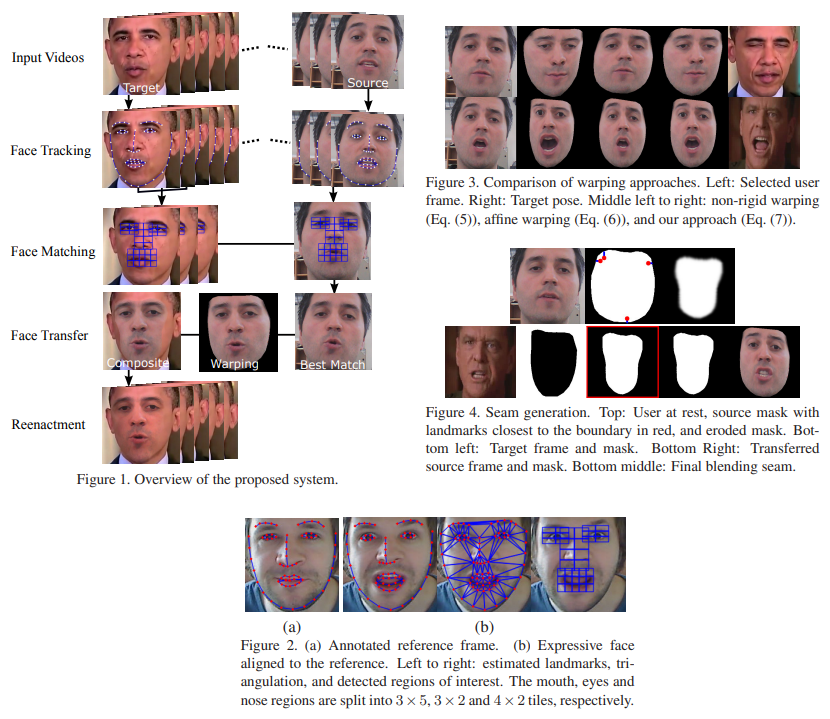
\includegraphics[width=0.80\textwidth]{img/ch1m4.png} 
\caption{Garrido P 等人一种基于图像的面部重建系统}
\label{Test}
\end{figure}

同样也是 Garrido P 等人\cite{garrido2015vdub},考虑到在许多国家,外国电影和电视作品被配音,即演员的原声被配音演员用该国自己的语言所说的翻译代替,配音是一个复杂的过程,需要特定的翻译和准确定时的朗诵,以使新音频至少粗略地贴合视频中的嘴巴动作。然而,由于原作和配音语言中的音素和视位序列不同,视频与音频的匹配永远不会完美,这是视觉不适的主要来源,在本文中,研究者提出了一种系统来改变视频中演员的嘴部动作,使其与新的音轨相匹配。其研究建立在对配音和目标演员的 3D 面部表演、照明和反照率的高质量单目捕捉的基础上,并结合使用音频分析和时空检索方法来合成一个新的照片般逼真的渲染和高度详细的 3D 形状嘴区域模型来替换目标性能。

\begin{figure}[htb]
\centering 
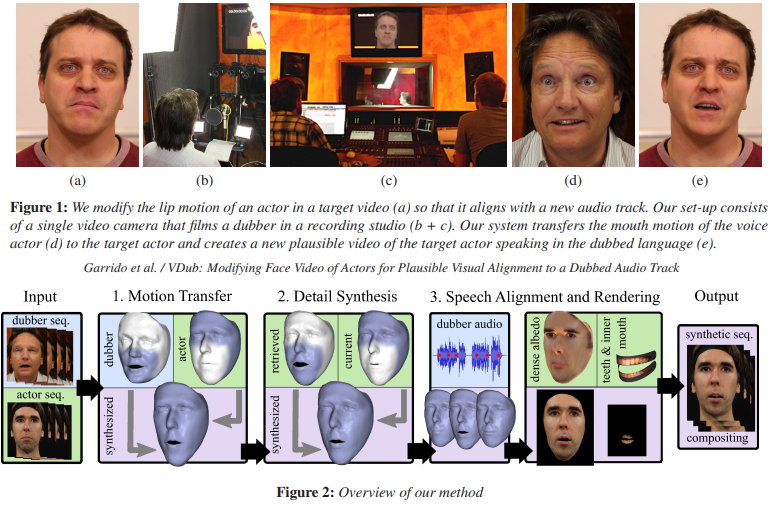
\includegraphics[width=0.70\textwidth]{img/ch1m5.png} 
\caption{Garrido P 等人提出了一种系统来改变视频中演员的嘴部动作,使其与新的音轨相匹配}
\label{Test}
\end{figure}

而 Nirkin Y 等人\cite{nirkin2018face}的研究让我们知道即使人脸图像不受约束且任意配对,它们之间的人脸交换实际上也非常简单。为此,该研究做出以下贡献。 (a) 没有像其他人之前提出的那样为人脸分割定制系统,而是展示了标准的全卷积网络 (FCN) 可以实现非常快速和准确的分割,前提是它在足够丰富的示例集上进行训练。为此,描述了新的数据收集和生成例程,这些例程提供了具有挑战性的分割人脸示例。 (b) 使用该研究的分割在前所未有的条件下实现强大的面部交换。 (c) 与以前的工作不同,该研究的交换足够强大,可以进行广泛的定量测试。为此,研究者使用野外标记人脸 (LFW) 基准测试并测量对象内和对象间人脸交换对识别的影响。研究表明,其受试者内部交换的面孔仍然与其来源一样可识别,证明了我们方法的有效性。与众所周知的感知研究一致,而更好的面部交换会产生不太可识别的主体间结果。这是第一次在机器视觉系统中定量证明这种效果。

\begin{figure}[htb]
\centering 
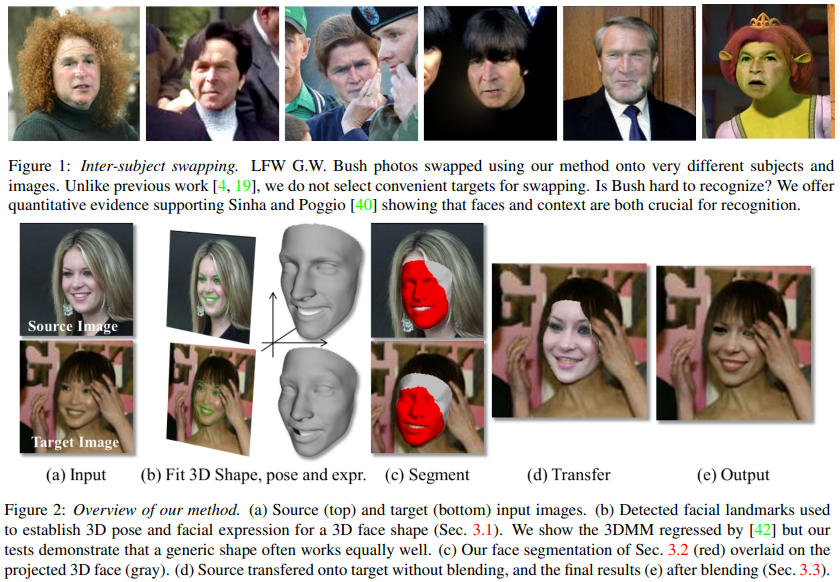
\includegraphics[width=0.70\textwidth]{img/ch1m6.png} 
\caption{Nirkin Y 用分割的思路促进换脸}
\label{Test}
\end{figure}

\subsubsection{现在根据深度学习所进行的脸部伪造技术}

由于过往图形学在面对伪造人类脸部技术有着极大的成本等诸多因素,从而导致该技术很难普遍的进行应用。然而自进入人工智能与机器学习所带动的深度学习热潮下,深度伪造技术在此之后有着非常快速的进展,此时许多研究者们开始关心其深度学习在人类脸部进行替换等应用技术。比如 Lu Z 等人 \cite{lu2017recent}则该研究领域所涉及传统方法和高级深度学习方法的典型人脸合成工作进行了全面回顾。特别是,Generative Adversarial Net (GAN) 被突出显示以生成照片般逼真和身份保持的结果。此外,还详细介绍了公开可用的数据库和评估指标。

\begin{figure}[htb]
\centering 
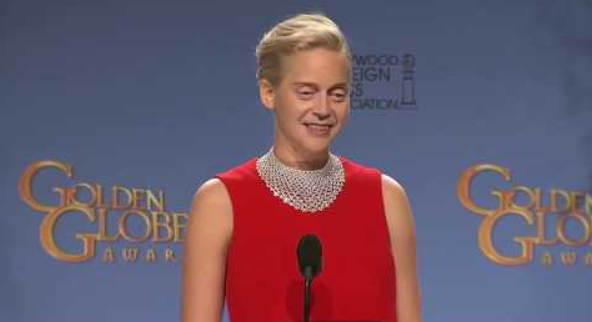
\includegraphics[width=0.40\textwidth]{img/ch1m7.png} 
\caption{FaceSwap 的 Jennifer Lawrence/Steve Buscemi FaceSwap using the Villain model}
\label{Test}
\end{figure}

当中 FaceSwap \cite{list1101} 是较早的一种利用深度学习来识别和交换图片和视频中的人脸的工具的 GitHub 开源项目,为具有多平台 Deepfakes 软件,其技术由 Tensorflow、Keras 和 Python 提供支持,并在 Windows、macOS 和 Linux 上运行。

该原理为在训练模型期间,去训练两个有共享权重参数的自动编码器,并让其两编码器获得有人类脸部重建效果的能力,其后在所谓换脸阶段,交换两解码器,使之有人类脸部交换的效果。重点在于此行为仅仅需要被窜改目标人物的脸部图像与原人物脸部图像即可进行模型的训练,与过往的成本相比,已大大降低其交换人类脸部成本,但此过程也需要一定的训练模型的基础知识与技术,不然其生成器所产生的品质是很可能达不到理想的成果,此 Deepfakes 生成概念可以从 Li XR 等人 \cite{2021496}所整理的工作总结看到。由于上述诸多原因,研究者们开始注意在生成对抗模型上的混合应用,

\begin{figure}[htb]
\centering 
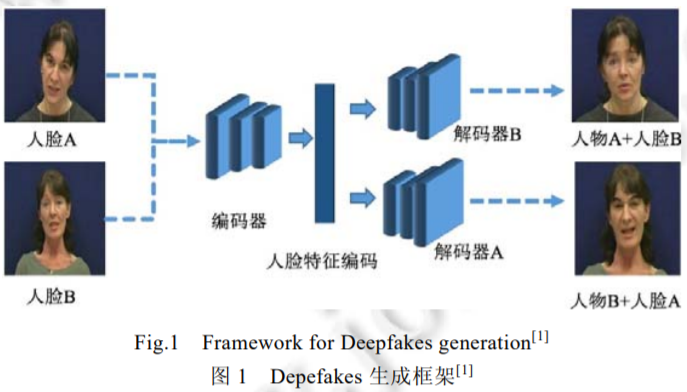
\includegraphics[width=0.60\textwidth]{img/ch1m8.png} 
\caption{Deepfakes 框架}
\label{Test}
\end{figure}

而所谓的生成对抗模型是源于 Goodfellow, I 等人 \cite{goodfellow2014generative}的工作,其研究者提出了一个通过对抗过程估计生成模型的新框架,该研究同时训练两个模型:一个生成模型 G 捕获数据分布,一个判别模型 D 估计样本来自训练数据而不是 G 的概率。 G 的训练过程是最大化 D 出错的概率。这个框架对应于一个极小极大的两人游戏,在任意函数 G 和 D 的空间中,存在唯一解,G 恢复训练数据分布,D 处处等于 1/2。在 G 和 D 由多层感知器定义的情况下,整个系统可以通过反向传播进行训练。在训练或生成样本期间,不需要任何马尔可夫链或展开的近似推理网络,实验通过对生成的样本进行定性和定量评估,证明了框架的潜力。而所谓的  Faceswap-GAN 混合 GAN 的深部伪造技术,其模型加入了判别器的对抗损失函数,另外再生成的部分对其生成的图像与原本的图像进行相似程度判断,该过程的好处在于会让生成的图像品质提高,且此模型也为了眼珠转动的部分加入了对应的感知损失函数。综上所述,我们可以知道因为 GAN 模型加入了该领域的发展后,使深度伪造技术的成本降低,仿造人类的换脸技术因此变得更加逼真,同时也使此技术流行起来。

\begin{figure}[htb]
\centering 
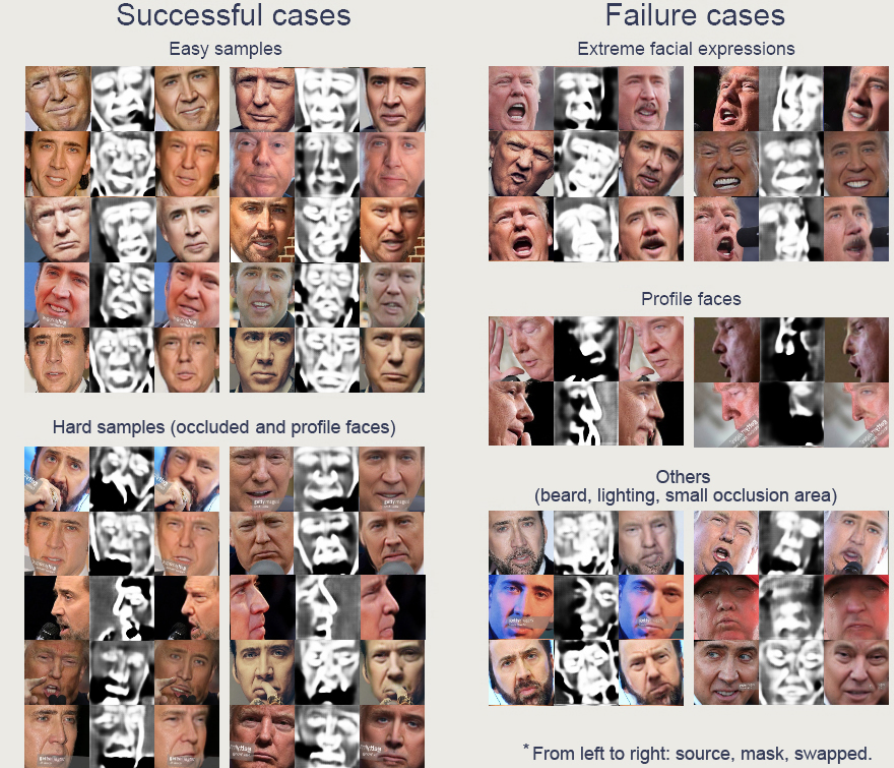
\includegraphics[width=0.60\textwidth]{img/ch1m9.png} 
\caption{Faceswap-GAN 展示了 v2 GAN 生成的 160 个随机结果,带有自注意力机制}
\label{Test}
\end{figure}

而 Korshunova 等人\cite{korshunova2017fast} 将所谓的深度伪造的换脸问题视为风格迁移问题,他们训练一个卷积神经网络,运用对非结构化的图像进行学习,其研究考虑图像中的人脸交换问题,其中输入身份被转换为目标身份,同时保留姿势、面部表情和照明,为了执行这种映射,研究者使用经过训练的卷积神经网络从他/她的照片的非结构化集合中捕获目标身份的外观,此方法是通过在风格转移方面构建人脸交换问题来实现的,其目标是用另一个风格来渲染图像。基于该领域的最新进展,研究者设计了一种新的损失函数,使网络能够产生高度逼真的结果,通过将神经网络与简单的预处理和后处理步骤相结合,研究者的目标是让面部交换实时工作,无需用户输入。另外 Nirkin Y 等人 \cite{nirkin2019fsgan}则提出了人脸交换 GAN (FSGAN) 用于人脸交换和重演,与以前的工作不同,FSGAN 与主题无关,可以应用于成对的面孔,而无需对这些面孔进行培训。为此,研究者描述了一些技术贡献,其推导出了一种新颖的基于循环神经网络 (RNN) 的面部重演方法,该方法可针对姿势和表情变化进行调整,并可应用于单个图像或视频序列,对于视频序列,我们引入了基于重演、Delaunay 三角剖分和重心坐标的人脸视图的连续插值,而被遮挡的人脸区域由人脸补全网络处理。最后,研究者使用人脸融合网络无缝融合两张脸,同时保留目标肤色和光照条件。该网络使用一种新颖的泊松混合损失,它将泊松优化与感知损失相结合。该研究将其方法与现有的最先进系统进行比较,并显示研究的结果在质量和数量上都优越。

同时也可以看到单纯窜改人类脸部属性与虚拟的人类脸部的 GAN 技术应用。比如 Choi Y 等研究者提出了 StarGAN \cite{choi2018stargan},这是一种新颖且可扩展的方法,可以仅使用单个模型为多个域执行图像到图像的转换,StarGAN 的这种统一模型架构允许在单个网络中同时训练具有不同域的多个数据集。与现有模型相比,这导致 StarGAN 具有卓越的翻译图像质量,以及将输入图像灵活翻译到任何所需目标域的新颖能力,研究者凭经验证明了其方法在面部属性转移和脸部表情合成任务上的有效性。 Zhang H 等人提出的 Stackgan \cite{zhang2018stackgan++} ,其研究者提出了一种用于文本到图像合成的两阶段生成对抗网络架构 StackGAN-v1,Stage-I GAN 根据给定的文本描述勾勒出对象的原始形状和颜色,产生低分辨率图像,Stage-II GAN 将 Stage-I 结果和文本描述作为输入,并生成具有照片般逼真细节的高分辨率图像,其次,针对有条件和无条件的生成任务提出了一种先进的多阶段生成对抗网络架构 StackGAN-v2。研究者的 StackGAN-v2 由树状结构中的多个生成器和判别器组成;从树的不同分支生成对应于同一场景的多个尺度的图像,StackGAN-v2 通过联合逼近多个分布,显示出比 StackGAN-v1 更稳定的训练行为。大量实验表明,所提出的堆叠生成对抗网络在生成照片般逼真的图像方面明显优于其他最先进的方法。Karras T 等人所提出 PGAN \cite{karras2017progressive} 的描述了一种用于生成对抗网络的新训练方法。关键思想是逐步增长生成器和判别器:从低分辨率开始,研究者添加了新的层,随着训练的进行,对越来越精细的细节进行建模。这既加快了训练的速度,又极大地稳定了训练,使研究者能够生成质量前所未有的图像,例如 1024\^2 的 CelebA 图像,其研究者还提出了一种简单的方法来增加生成图像的变化,并在无监督 CIFAR10 中实现 8.80 的创纪录初始分数。此外,研究者描述了几个实现细节,这些细节对于阻止生成器和判别器之间的不健康竞争很重要。最后,该研究建议在图像质量和变化方面评估 GAN 结果的新指标,作为额外的贡献,研究者构建了更高品质的 CelebA 资料集版本。这些一系列的 GAN 技术也可以生成虚拟人物的人类面部图像。

另外则是 Grigory 等人\cite{antipov2017face}运用 Mirza M 等人的 conditional-GAN \cite{mirza2014conditional} ,其在这项工作中,Mirza M 等研究者介绍了生成对抗网络的条件版本,它可以通过简单地输入数据 y 来构建,我们希望同时对生成器和判别器进行条件处理。该研究展示了该模型可以生成以类标签为条件的 MNIST 数字。其研究还说明了该模型如何用于学习多模态模型,并提供了图像标记应用的初步示例,其中研究者演示了该方法如何生成不属于训练标签的描述性标签。 Grigory 等人则在此基础上提出了基于 GAN 的自动人脸老化方法。与以前使用 GAN 来改变面部属性的工作相反,研究者特别强调在他/她的面部老化版本中保留原始人的身份。为此,该研究引入了一种新的方法来优化 GAN 的潜在向量的“身份保持”。通过最先进的人脸识别和年龄估计解决方案对产生的老化和恢复活力的人脸图像进行客观评估,证明了所提出方法的巨大潜力。
还有 Huang R 等人\cite{huang2017beyond}提出了一种双路径生成对抗网络(TP-GAN),用于通过同时感知全局结构和局部细节来进行逼真的正面视图合成。除了常用的全局编码器-解码器网络之外,还提出了四个具有里程碑意义的补丁网络来处理局部纹理。除了新颖的架构外,研究者通过引入对抗性损失、对称性损失和身份保持损失的组合来很好地约束这个不适定问题,组合的损失函数利用正面人脸分布和预训练的判别式深度人脸模型来指导从侧面看正面视图的身份保持推断。与之前主要依赖中间特征进行识别的深度学习方法不同,该研究的方法直接利用合成的身份保持图像来完成人脸识别和属性估计等下游任务,其实验结果表明,该研究的方法不仅提供了令人信服的感知结果,而且在大姿势人脸识别方面也优于最先进的结果。综上所述因为 GAN 技术的应用于深度伪造领域使其成果越来越真实,从而引来该技术滥用在负面用途开端。

\subsection{人类脸部的表情伪造}

所謂的人类脸部的表情伪造在於不去對該目標人物去進行替換,讓其他不同臉部表情的特徵來改變目標人物的表情。

比如 Thies J 等人 \cite{thies2015real} 所提出的了一种将面部表情从源视频中的演员实时传输到目标视频中的演员的方法,从而能够对目标演员的面部表情进行临时控制。其方法的新颖之处在于将面部变形和细节的转移和逼真的重新渲染到目标视频中,新合成的表情与真实视频几乎没有区别。为了实现这一点,该研究使用商品 RGB-D 传感器实时准确地捕捉源对象和目标对象的面部表现,对于每一帧,研究者将身份、表情和皮肤反射率的参数模型与输入颜色和深度数据联合拟合,并重建场景照明。对于表达式转移,该研究计算参数空间中源表达式和目标表达式之间的差异,并修改目标参数以匹配源表达式。一个主要挑战是将合成的目标人脸重新渲染到相应的视频流中,这需要仔细考虑照明和阴影设计,两者都必须与现实世界环境相对应。研究者在现场设置中演示了其方法,并修改了视频会议来源,以便实时匹配不同人(例如翻译)的面部表情。另外也是 Thies J 等人 \cite{thies2016face2face}提出了 Face2Face,这是一种用于对单目目标视频序列(例如 Youtube 视频)进行实时面部重演的新颖方法,源序列也是单目视频流,使用商品网络摄像头实时捕获。其目标是通过源演员为目标视频的面部表情制作动画,并以照片般逼真的方式重新渲染经过处理的输出视频。为此,研究者首先通过基于非刚性模型的捆绑解决了从单目视频中恢复面部身份的约束不足问题。同时运行时使用密集的光度一致性测量来跟踪源视频和目标视频的面部表情。然后通过源和目标之间的快速有效的变形传递来实现重演,从目标序列中检索与重新定位的表情最匹配的嘴巴内部,并对其进行扭曲以产生准确的拟合。最后,研究者令人信服地在相应的视频流之上重新渲染合成的目标人脸,使其与现实世界的照明无缝融合。另外还提出 HeadOn 这是第一个实时的源到目标重演方法,用于完整的人类肖像视频,可以传输躯干和头部运动、面部表情和眼睛注视。给定目标演员的简短 RGB-D 视频,其研究者自动构建个性化几何代理,该代理嵌入参数化头部、眼睛和运动学躯干模型。而一种新颖的实时重演算法使用此代理将捕获的运动从源演员逼真地映射到目标演员。在粗略的几何代理之上,研究者提出了一种基于视频的渲染技术,该技术通过与视图和姿势相关的纹理合成修改后的目标肖像视频,并在新颖的躯干和头部姿势下创建目标演员的照片般逼真的图像,面部表情和注视方向。为此,研究者建议对源演员的面部和躯干进行稳健的跟踪。

\begin{figure}[htb]
\centering 
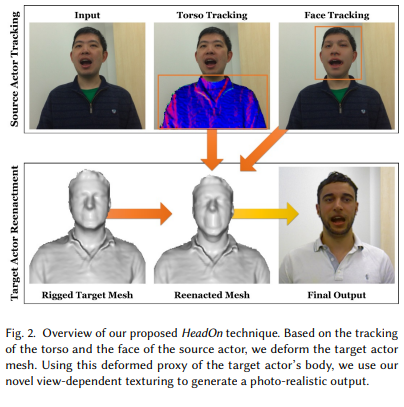
\includegraphics[width=0.60\textwidth]{img/ch1m10.png} 
\caption{HeadOn}
\label{Test}
\end{figure}

Kim H 等人 \cite{kim2018deep} 提出了一种新颖的方法,该方法仅使用输入视频就可以对肖像视频进行逼真的重新动画处理。与仅限于面部表情操作的现有方法相比,研究者率先将完整的 3D 头部位置、头部旋转、面部表情、眼睛注视和眨眼从源演员转移到目标的肖像视频演员,其方法的核心是具有新颖时空架构的生成神经网络。该网络将参数化人脸模型的合成渲染作为输入,并据此预测给定目标演员的照片般逼真的视频帧,这种从渲染到视频的传输的真实性是通过仔细的对抗训练来实现的,因此,研究者可以创建修改后的目标视频,以模仿合成创建的输入的行为。为了实现源到目标视频的重新动画,研究者使用从源视频中重建的头部动画参数渲染合成目标视频,并将其输入到训练好的网络中,从而完全控制目标,凭借自由重组源参数和目标参数的能力,研究者能够演示各种视频重写应用程序,而无需明确建模头发、身体或背景。例如,该研究可以使用交互式用户控制的编辑来重新制作完整的头部,并实现高保真视觉配音。为了证明其成果输出的高质量,研究者进行了一系列广泛的实验和评估,例如,用户研究表明该研究的视频编辑很难检测到。

Thies J 等人 \cite{thies2019deferred}探索了不完美的 3D 内容的使用,例如,从具有噪声和不完整表面几何的光度重建中获得,同时仍然旨在产生照片般逼真的(重新)渲染。为了解决这个具有挑战性的问题,研究者引入了延迟神经渲染,这是一种将传统图形管道与可学习组件相结合的图像合成新范例。具体来说,该研究提出了神经纹理,它是作为场景捕获过程的一部分进行训练的学习特征图。与传统纹理类似,神经纹理作为贴图存储在 3D 网格代理之上;然而,高维特征图包含更多信息,可以通过我们新的延迟神经渲染管道进行解释,神经纹理和延迟神经渲染器都是端到端训练的,即使原始 3D 内容不完美,我们也能够合成照片般逼真的图像。与传统的黑盒 2D 生成神经网络相比,研究者的 3D 表示使我们能够明确控制生成的输出,并允许广泛的应用领域。例如,该研究可以合成时间一致的视频重新渲染记录的 3D 场景,因为研究者表示固有地嵌入在 3D 空间中。通过这种方式,可以利用神经纹理在静态和动态环境中以实时速率连贯地重新渲染或操作现有视频内容。该研究在几个关于新视图合成、场景编辑和面部重演的实验中展示了其方法的有效性,并与利用标准图形管道和传统生成神经网络的最先进方法进行了比较。

Suwajanakorn S 等人 \cite{10.1145/3072959.3073640}提出了根据循环神经网络来建立人类面部嘴型与人类语音资料的对应,并利用美国总统巴拉克奥巴马的音频,研究者合成了一段高质量的他讲话的视频,并具有准确的口型同步,并合成到目标视频剪辑中,一个循环神经网络在他每周的演讲视频中经过数小时的训练,可以学习从原始音频特征到嘴形的映射。给定每个时刻的嘴巴形状,研究者合成高质量的嘴巴纹理,并将其与适当的 3D 姿势匹配合成,以改变他在目标视频中所说的内容,以匹配输入音轨。其方法产生逼真的结果。

Zakharov E 等人 \cite{Zakharov_2019_ICCV}研展示了一个具有人物特写镜头画面的图像合成。它在大型视频数据集上执行冗长的元学习,然后能够将以前看不见的人的神经说话头模型的少量和一次性学习构建为具有高容量生成器和鉴别器的对抗性训练问题。至关重要的是,该系统能够以特定于人的方式初始化生成器和判别器的参数,因此尽管需要调整数千万个参数,但训练可以仅基于几张图像并快速完成。其研究表明,这种方法能够学习高度逼真和个性化的新人说话头部模型,甚至是肖像画。

类似的还有 Fried O 等人\cite{10.1145/3306346.3323028} 提出了一种新颖的方法来编辑说话头视频的脚本,以生成逼真的输出视频,其中说话者的对话已被修改,同时保持无缝的视听流(即没有跳转)。其方法使用音素、视位、3D 面部姿势和几何形状、反射率、表情和每帧场景照明自动注释输入的说话头视频,要编辑视频,用户只需编辑脚本,然后优化策略选择输入语料库的片段作为基础材料。与所选片段对应的注释参数无缝拼接在一起,并用于生成中间视频表示,其中脸部的下半部分用参数化脸部模型渲染,最后该循环视频生成网络将此表示转换为与编辑后的文字记录相匹配的逼真视频。研究者展示了各种各样的编辑,例如单词的添加、删除和更改,以及令人信服的语言翻译和完整的句子合成。

Averbuch-Elor H 等人 \cite{10.1145/3130800.3130818}提出了一种自动为静止肖像制作动画的技术,使照片中的主体能够栩栩如生并表达各种情感,该研究使用(不同主题的)驾驶视频,并开发了将驾驶视频中主题的表现力转移到目标肖像的方法。与之前需要目标面部的输入视频来重现面部表现的工作相比,我们的技术仅使用单个目标图像,研究者通过模仿驾驶视频中的面部变换的 2D 扭曲对目标图像进行动画处理。由于单独的经线不能承载面部的全部表现力,因此研究者添加了通常与面部表情相关的精细动态细节,例如折痕和皱纹。此外,该研究对隐藏在输入目标面部中的区域产生幻觉,尤其是在嘴巴内。其技术产生了反应式配置文件,静止图像中的人可以自动与他们的观众互动,最后展示了该研究在互联网上的大量静态肖像上运行的技术。

Lample G 等人 \cite{NIPS2017_3fd60983} 介绍了一种新的编码器-解码器架构,该架构经过训练,可通过直接在潜在空间中解开图像的显著信息和属性值来重建图像。因此,经过训练,其模型可以通过改变属性值来生成输入图像的不同真实版本。通过使用连续的属性值,研究者可以选择在生成的图像中可以感知多少特定属性。此属性可以允许用户使用滑动旋钮修改图像的应用程序,例如混合控制台上的推子,以更改肖像的面部表情或更新某些对象的颜色。与主要依赖于通过在训练时更改属性值来训练像素空间中的对抗性网络的最先进技术相比,该研究的方法产生了更简单的训练方案并且可以很好地扩展到多个属性。其提供的证据表明,该模型可以显著改变属性的感知价值,同时保持图像的自然性。

\subsection{人类语音的伪造}

所谓的语音伪造则是根据人工智能的发展下利用相关的技术对人类语音进行合成,其技术分为两大部分,其一为所谓的语音变换(Voice Conversion),其二为文本对语音资料的合成 (Text-to-speech),前者意义为将人的说话的音调改变为目标人物的音调,后者则是搜集大量的语音与对应文本资料来完成指定语音资讯的输出。这些成果除了可以让一些人无法辨识出是否为当事人,跟甚者能够欺骗过一些语音辨识系统。过往语音伪造都为高斯混合模型(Gaussian Mixture Model,GMM)与隐马尔可夫模型(Hidden Markov Model, HMM),但随人工智能等领域带动深度学习的技术改进,在这块语音伪造技术则有着明显的突破。

其 Van Den Oord A 等人 提出 WaveNet,一种用于生成原始音频波形的深度神经网络。该模型是完全概率和自回归的,每个音频样本的预测分布都以所有先前的样本为条件;尽管如此,该研究证明它可以在每秒数万个音频样本的数据上进行有效训练。当应用于文本到语音时,它产生了最先进的性能,人类听众认为它比英语和普通话的最佳参数和连接系统听起来更自然。单个 WaveNet 可以以相同的保真度捕获许多不同说话者的特征,并且可以通过调节说话者身份在它们之间切换。当训练为音乐建模时,我们发现它会生成新颖且通常高度逼真的音乐片段。其研究者还表明它可以用作判别模型,为音素识别返回有希望的结果。

\begin{figure}[htb]
\centering 
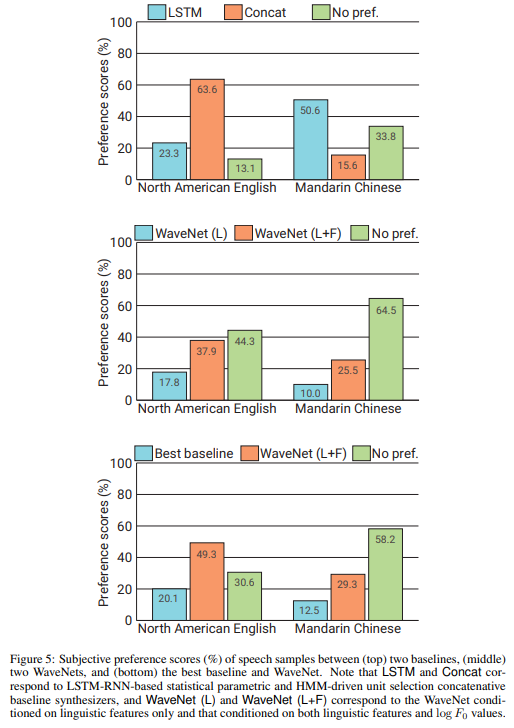
\includegraphics[width=0.60\textwidth]{img/ch1m11.png} 
\caption{Van Den Oord A 等人 提出 WaveNet}
\label{Test}
\end{figure}

\subsection{商用化软体产品与现有开源工具}





%\begin{itemize}
%\item [-][7,7] 空间卷积到 1*1*2048 然后一维卷积到 1*1*128
%\item [-]池化层到 1*1*2048 然后一维卷积到 1*1*128
%\end{itemize}



%\begin{itemize}
%\item Calculus
%\item Linear Algebra
%\item Basic Computer Concepts
%\end{itemize}

%\begin{description}
% \item[First] \hfill \\
% The first item
% \item[Second] \hfill \\
% The second item
% \item[Third] \hfill \\
% The third etc \ldots
%\end{description}
